
\documentclass[border=5pt]{standalone}
\usepackage[utf8]{inputenc}
\usepackage[T1]{fontenc}
\usepackage{amsmath,amssymb}
\usepackage{tikz}
\usetikzlibrary{arrows.meta,shapes.misc,calc}
\renewcommand{\familydefault}{\sfdefault}
\tikzset{
  ptcross/.style={cross out,draw,thick,minimum size=1.6mm,inner sep=0pt},
  vec/.style={->,thick,>={Stealth[length=2.6mm]}},
  vecu/.style={vec,color=blue!70!black},
  vecv/.style={vec,color=red!75!black},
  vecw/.style={vec,color=green!45!black},
  grid/.style={gray!35,thin},
}
\newcommand{\Vj}[1]{\overrightarrow{\text{#1}}}
\newcommand{\pt}[4]{\node[ptcross] at (#1,#2) {}; \node[anchor=#4,inner sep=2pt] at (#1,#2) {$#3$};}
\begin{document}
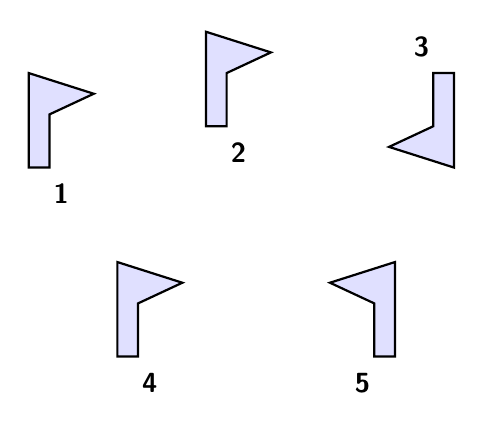
\begin{tikzpicture}[x=0.75cm,y=0.75cm]
\begin{scope}[shift={(0,0)},rotate=0,xscale=1]\draw[thick,fill=blue!12] (0,0) -- (0,1.6) -- (1.1,1.25) -- (0.35,0.9) -- (0.35,0) -- cycle;\node at (0.55,-0.45) {\bfseries 1};\end{scope}
\begin{scope}[shift={(3,0.7)},rotate=0,xscale=1]\draw[thick,fill=blue!12] (0,0) -- (0,1.6) -- (1.1,1.25) -- (0.35,0.9) -- (0.35,0) -- cycle;\node at (0.55,-0.45) {\bfseries 2};\end{scope}
\begin{scope}[shift={(7.2,1.6)},rotate=180,xscale=1]\draw[thick,fill=blue!12] (0,0) -- (0,1.6) -- (1.1,1.25) -- (0.35,0.9) -- (0.35,0) -- cycle;\node at (0.55,-0.45) {\bfseries 3};\end{scope}
\begin{scope}[shift={(1.5,-3.2)},rotate=0,xscale=1]\draw[thick,fill=blue!12] (0,0) -- (0,1.6) -- (1.1,1.25) -- (0.35,0.9) -- (0.35,0) -- cycle;\node at (0.55,-0.45) {\bfseries 4};\end{scope}
\begin{scope}[shift={(6.2,-3.2)},rotate=0,xscale=-1]\draw[thick,fill=blue!12] (0,0) -- (0,1.6) -- (1.1,1.25) -- (0.35,0.9) -- (0.35,0) -- cycle;\node at (0.55,-0.45) {\bfseries 5};\end{scope}

\end{tikzpicture}
\end{document}
